\thispagestyle{toancuabinone}
\pagestyle{toancuabi}
\everymath{\color{toancuabi}}
\blfootnote{$^1$\color{toancuabi}Trường Liên cấp Hội nhập Quốc tế iSchool Quảng Trị.}
\graphicspath{{../toancuabi/pic2/}}
\begingroup
\AddToShipoutPicture*{\put(0,616){\includegraphics[width=19.3cm]{../bannertoancuabi}}}  
\AddToShipoutPicture*{\put(110,525){\includegraphics[scale=1]{../tieude10.pdf}}}  
\centering
\endgroup
\vspace*{185pt} 

\begin{multicols}{2}
	\textbf{\color{toancuabi}Làm diều giấy}
	\vskip 0.1cm
	Còn gì tuyệt vời hơn khi được thả diều dưới bầu trời xanh và trong làn gió mát của những buổi chiều mùa hè oi ả. Bằng những kiến thức của bài ``Hình có trục đối xứng" và trí tưởng tượng phong phú của mình, em hãy tự làm ra cho mình một con diều đẹp đẽ với màu sắc rực rỡ nhé. Chúc em thành công!
	\begin{figure}[H]
		\vspace*{-5pt}
		\centering
		\captionsetup{labelformat= empty, justification=centering}
		\includegraphics[width= 1\linewidth]{1}
		\caption{\small\textit{\color{toancuabi}Hình ảnh con diều (Ảnh: Internet).}}
		\vspace*{-10pt}
	\end{figure}
	\textit{Bước} $1$: Lấy một mảnh giấy để tạo thành thân diều. Nếu em mong muốn có một chiếc diều thật lớn, hãy ghép bốn mảnh giấy lại với nhau. Tuy nhiên phải dán bốn mảnh giấy lại sao cho thật khít, thật đều và phải dán băng dính ở cả hai mặt tại chỗ nối. Vết ghép phải cũng phải thật chắc chắn để bảo đảm diều không bị bung ra khi thả.
	\begin{figure}[H]
		\vspace*{5pt}
		\centering
		\captionsetup{labelformat= empty, justification=centering}
		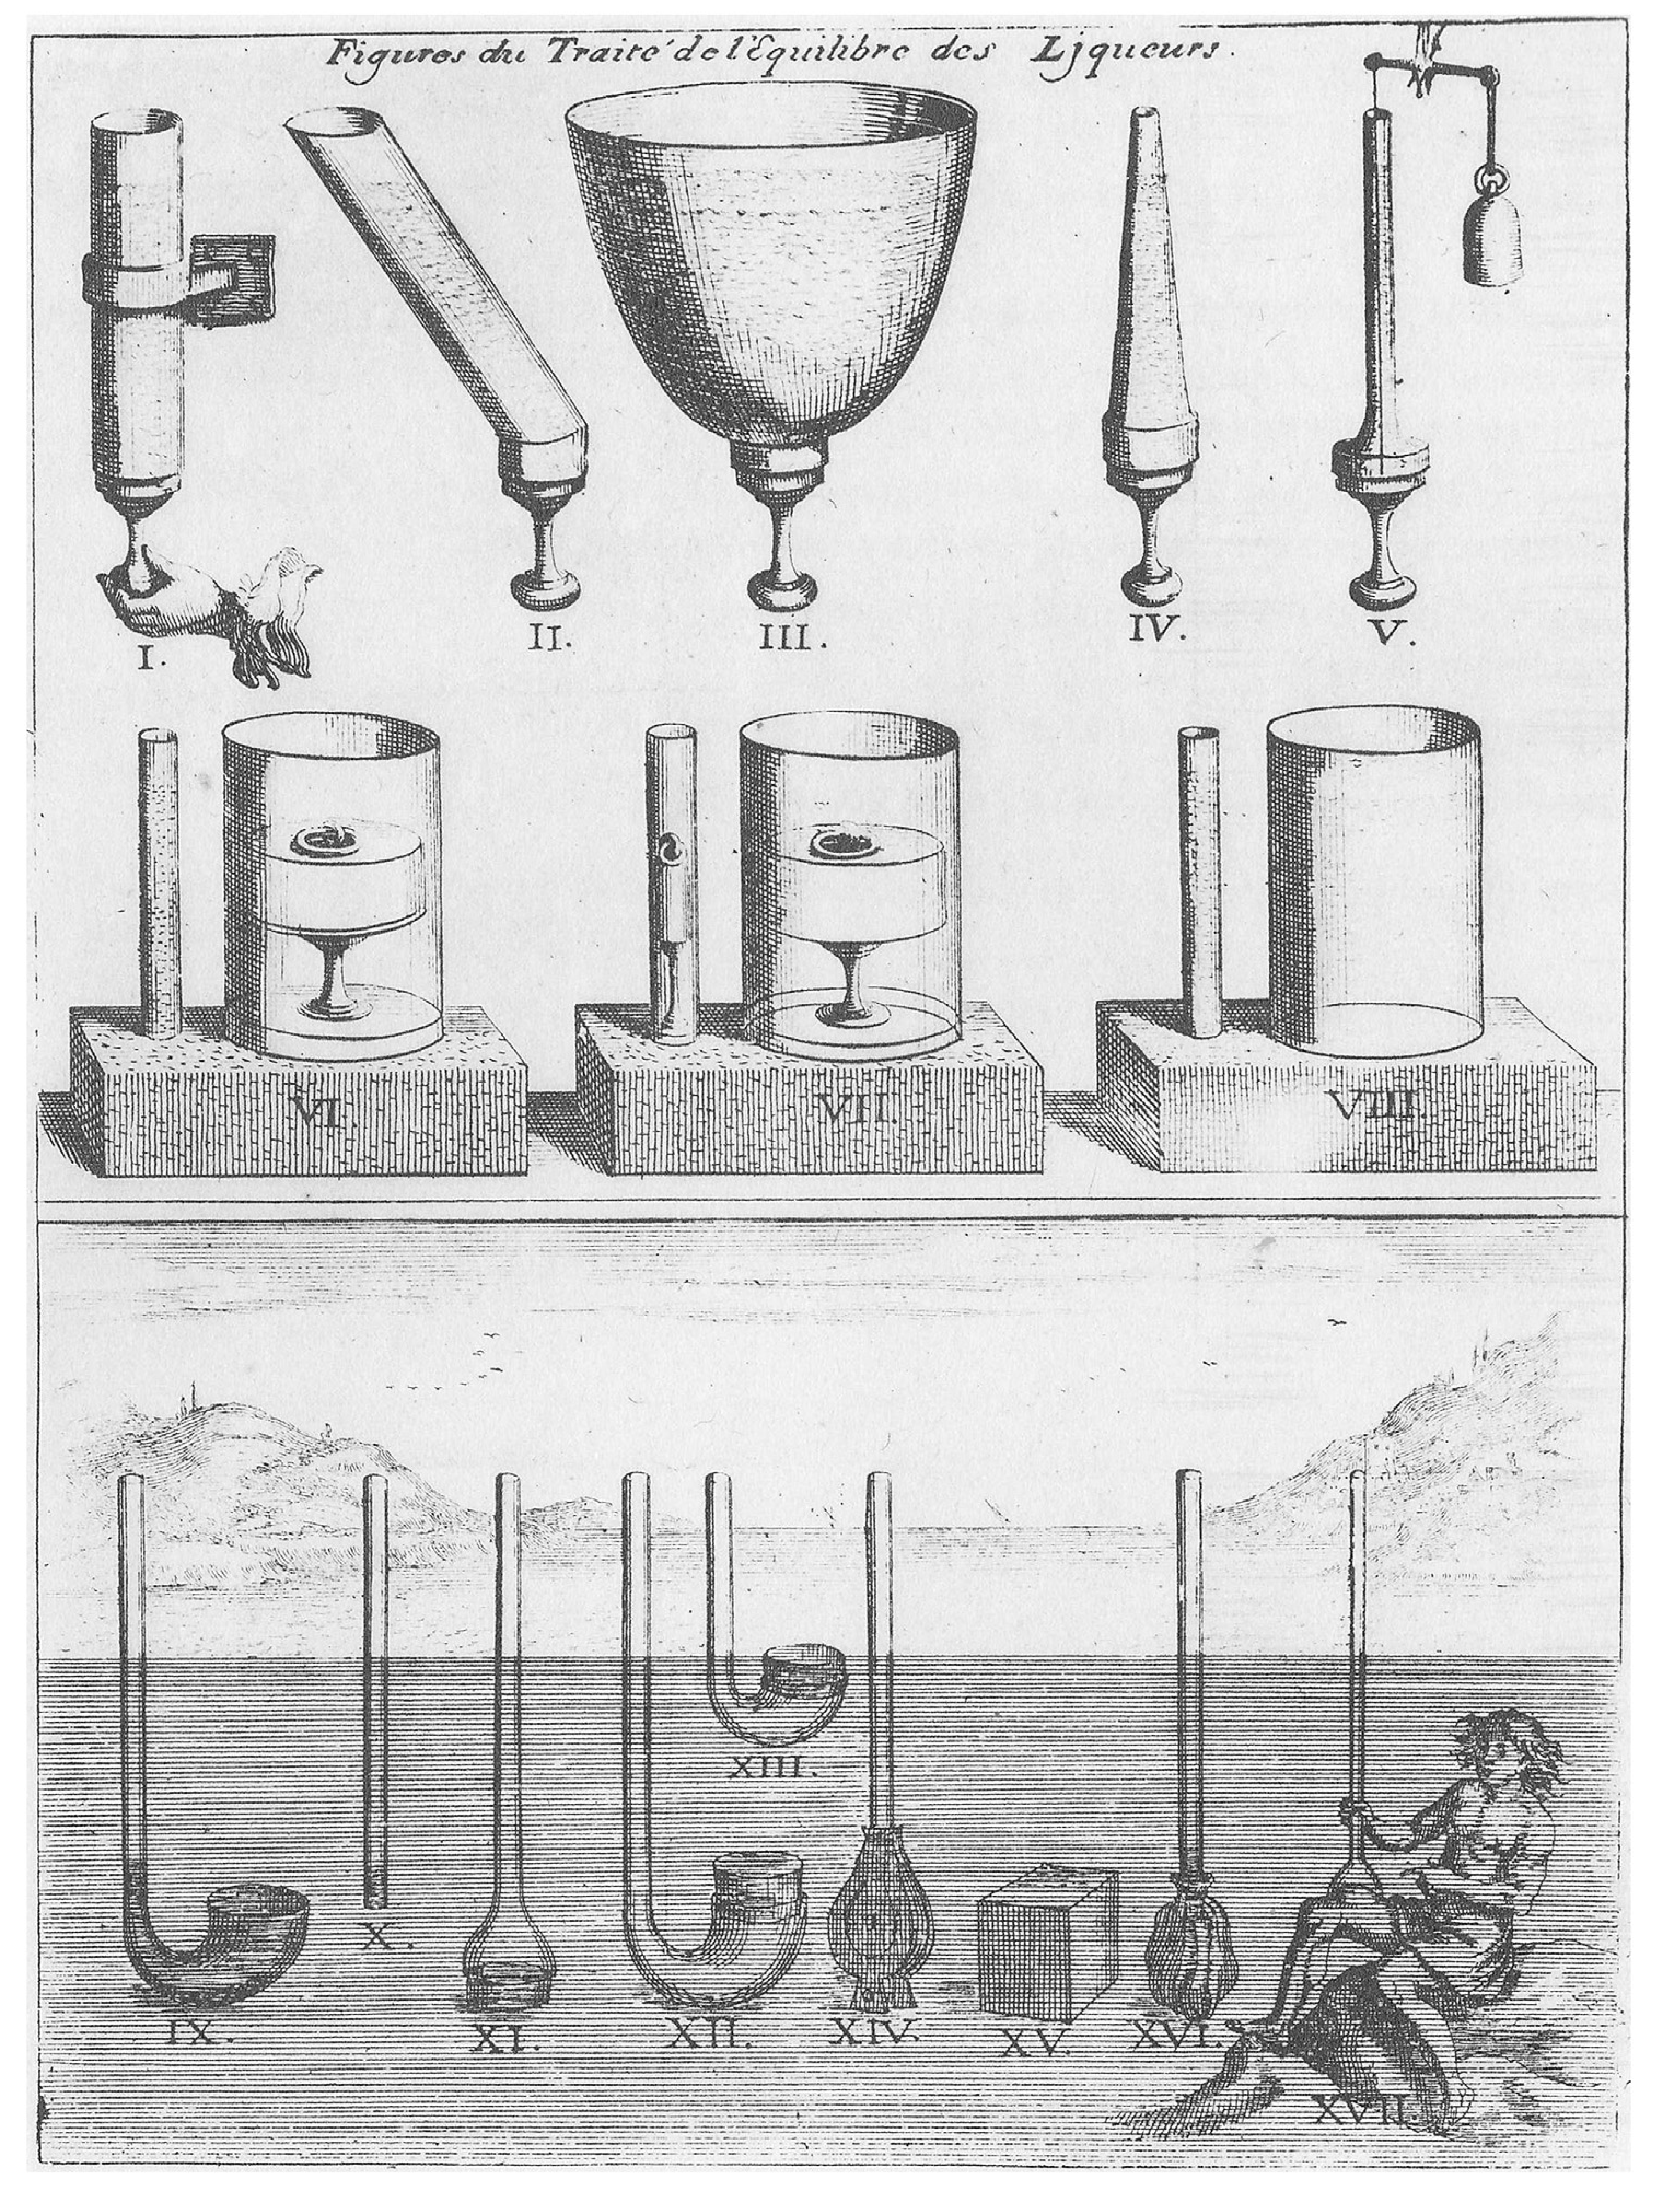
\includegraphics[width= 1\linewidth]{2}
		%		\caption{\small\textit{\color{toancuabi}Hình ảnh con diều (Ảnh: Internet).}}
		\vspace*{-10pt}
	\end{figure}
	\textit{Bước} $2$: Chia mảnh giấy thành $4$ phần, vẽ một hình kim cương trên giấy sao cho phần đáy chiếm $3/4$, còn phần đầu chiếm $1/4$ chiều dài tờ giấy. Sau đó, cắt bỏ những phần giấy thừa bên ngoài như hình.
	\begin{figure}[H]
		\vspace*{-5pt}
		\centering
		\captionsetup{labelformat= empty, justification=centering}
		\includegraphics[width= 1\linewidth]{3}
		\vspace*{-10pt}
	\end{figure}
	\textit{Bước} $3$: Buộc hai que tre với nhau theo hình thánh giá. Để chắc chắn rằng vết buộc nằm đúng vị trí chính giữa, hãy ướm thử lên giấy. Chú ý rằng không nên sử dụng dây thừng để buộc mối nối giữa hai que tre vì sẽ gây cộm, cũng không được sử dụng sợi cước vì quá trơn. Dây sử dụng để buộc mối nối cần mảnh, chắc và không trơn (ví dụ như sợi dây dù, chỉ may,...).
	\begin{figure}[H]
		\vspace*{-5pt}
		\centering
		\captionsetup{labelformat= empty, justification=centering}
		\includegraphics[width= 1\linewidth]{4}
		\vspace*{-10pt}
	\end{figure}
	\textit{Bước} $4$: Đục lỗ ở $4$ góc hình kim cương để luồn dây xuyên qua, cố định phần khung tre với phần thân giấy. Để vết buộc tránh bị xê dịch, em có thể khứa rãnh trên thanh tre và cố định sợi chỉ luồn trong rãnh đấy.
	\begin{figure}[H]
		\vspace*{-5pt}
		\centering
		\captionsetup{labelformat= empty, justification=centering}
		\includegraphics[width= 1\linewidth]{5}
		\vspace*{-10pt}
	\end{figure}
	\textit{Bước} $5$: Buộc một sợi dây (dài hơn thanh nan ngang) vắt ngang diều (gọi là sợi dây số $1$). Sau đó, lấy một sợi dây dài khác buộc vào chính giữa sợi dây số $1$ để làm dây thả diều.
	\begin{figure}[H]
		\vspace*{-5pt}
		\centering
		\captionsetup{labelformat= empty, justification=centering}
		\includegraphics[width= 1\linewidth]{6}
		\vspace*{-10pt}
	\end{figure}
	\textit{Bước} $6$: Dán thêm các dải giấy màu ở các góc của con diều (trừ góc đầu) để con diều thêm nổi bật.
	\begin{figure}[H]
		\vspace*{-5pt}
		\centering
		\captionsetup{labelformat= empty, justification=centering}
		\includegraphics[width= 1\linewidth]{7}
		\vspace*{-10pt}
	\end{figure}
	\textit{Bước} $7$: Em hãy tìm một khu vực rộng rãi, thoáng mát và có gió để thả diều. Khi thả diều nên có hai người để phối hợp, một người cầm cuộn dây để giật diều còn một người chạy đà để thả diều. Chú ý phải chạy ngược chiều gió thì con diều mới có thể bay lên.
	\vskip 0.1cm
	\textbf{\color{toancuabi}Tài liệu tham khảo}
	\vskip 0.1cm
	\url{https://www.butsaigon.com/lam-do-hand}\\
	\url{made/huong-dan-cach-lam-dieu-giay.html}
\end{multicols}
\newpage
\graphicspath{{../toancuabi/pic/}}
\begingroup
\AddToShipoutPicture*{\put(156,675){\includegraphics[scale=1]{../tieudea.pdf}}}  
\centering
\endgroup
\vspace*{30pt} 
\begin{multicols}{2}
	Thám tử Xuân Phong có một lần bị lạc trên một hòn đảo xa tít tắp giữa đại dương sau một vụ đắm tàu. Khi tỉnh dậy, thám tử biết mình đã được cứu sống bởi một bộ tộc khá kỳ lạ. Người dân của bộ tộc được chia thành $3$ loại người -- người Thật thà, người Nói dối và người Phụ hoạ, hơn nữa ai cũng biết rõ về tất cả những người còn lại, ai là thuộc loại người nào. Sau khi Xuân Phong được chiêu đãi no nê bởi vị thủ lĩnh bộ lạc và được thay quần áo tinh tươm, tất cả $500$ thổ dân bộ tộc đứng thành hàng ngang trước mặt Xuân Phong để ra mắt chào mừng vị thám tử. Xuân Phong đưa ra câu hỏi sau cho họ: ``Trên hòn đảo này có phải là số người Thật thà nhiều hơn số người Nói dối hay không?". Các thổ dân lần lượt trả lời một cách dõng dạc  ``Không" hoặc ``Có" để tất cả mọi người còn lại đều nghe thấy. 
	\vskip 0.1cm
	Người Thật thà thì luôn nói thật, người Nói dối thì luôn nói dối, còn một người Phụ hoạ thì trả lời như đa số những người đã trả lời trước anh ta, còn nếu như số câu trả lời ``Có" và ``Không" trước đó mà bằng nhau thì người Phụ hoạ sẽ trả lời ``Có" hoặc ``Không" tuỳ ý. 
	\vskip 0.1cm
	Sau khi cả $500$ thổ dân đã trả lời xong, Xuân Phong thấy số câu trả lời ``Có" là $250$. Hỏi trong bộ tộc đó có nhiều nhất bao nhiêu người Phụ hoạ?
	\begin{figure}[H]
		\centering
		\vspace*{-5pt}
		\captionsetup{labelformat= empty, justification=centering}
		\includegraphics[width=1\linewidth]{xp}
%		\vspace*{5pt}
	\end{figure}
\end{multicols}
\vspace*{-10pt}
{\color{toancuabi}\rule{1\linewidth}{0.1pt}}
\begingroup
\AddToShipoutPicture*{\put(115,310){\includegraphics[scale=1]{../tieude11.pdf}}} 
\centering
\endgroup
\vspace*{50pt}

\begin{multicols}{2}
	$\pmb{1.}$ 	Trong ngày sinh nhật của mình, An mời $5$ người bạn tới nhà ăn bánh ga tô. An cắt cho người bạn thứ nhất $\frac{1}{6}$ chiếc bánh. Người bạn thứ hai được An cắt cho $\frac{1}{5}$ số bánh còn lại,
	\begin{figure}[H]
		\centering
		\vspace*{-10pt}
		\captionsetup{labelformat= empty, justification=centering}
		\includegraphics[width=0.6\linewidth]{Pi10_bai1}
		\vspace*{-5pt}
	\end{figure}
	người bạn thứ ba được An cắt cho $\frac{1}{4}$ số bánh còn lại sau khi đã lấy bánh cho người bạn thứ hai, người thứ tư được chia $\frac{1}{3}$ số bánh còn lại sau khi đã lấy bánh cho người bạn thứ ba. Phần bánh cuối cùng được An cắt làm đôi và chia đều với người bạn thứ năm. Hỏi ai đã được chia nhiều bánh nhất?
	\vskip 0.1cm
	$\pmb{2.}$ Tùng và Sơn cùng nhảy từ bờ xuống mặt nước và bơi về phía một hòn đảo.  Khi Sơn bơi được $40$ mét thì Tùng đã bơi đến được bờ của hòn đảo. Vừa chạm tới bờ, Tùng lại ngay lập tức bơi ngược lại và gặp lại Sơn vào thời điểm Sơn đã bơi thêm được $8$ mét nữa. Hỏi khoảng cách từ điểm xuất phát của hai bạn tới bờ hòn đảo là bao nhiêu?
	\begin{figure}[H]
		\centering
		\vspace*{5pt}
		\captionsetup{labelformat= empty, justification=centering}
		\includegraphics[width=1\linewidth]{Pi10_bai2}
		\vspace*{-15pt}
	\end{figure}
	$\pmb{3.}$ Một tấm bìa hình chữ nhật kích thước $5\times 9$ được cắt ra thành $10$ hình chữ nhật nhỏ với các cạnh là các số nguyên. Em hãy chỉ ra rằng trong số các hình được cắt ra này có hai hình kích thước giống hệt nhau.
	\begin{figure}[H]
		\centering
		\vspace*{-5pt}
		\captionsetup{labelformat= empty, justification=centering}
		\includegraphics[width=1\linewidth]{Pi10_bai3}
		\vspace*{-15pt}
	\end{figure}
	$\pmb{4.}$ Một nàng tiên đi tới một con suối nguồn với hai chiếc bình trên tay. Một chiếc bình có thể tích $5$ lít, còn chiếc kia có thể tích $4$ lít. Nước chảy ra từ suối nước theo hai dòng, một dòng mạnh hơn, còn dòng kia yếu hơn. Nàng tiên đặt đồng thời hai chiếc bình mỗi chiếc dưới một dòng nước.
	\begin{figure}[H]
		\centering
		\vspace*{-5pt}
		\captionsetup{labelformat= empty, justification=centering}
		\includegraphics[width=1\linewidth]{Pi10_bai4}
		\vspace*{-15pt}
	\end{figure}
	 Khi đã hứng đầy được một nửa chiếc bình nhỏ, nàng tiên đổi vị trí hai bình cho nhau. Và vô cùng ngạc nhiên, hai chiếc bình được hứng đầy vào cùng một lúc. Hỏi  dòng nước mạnh chảy mạnh hơn gấp mấy lần so với dòng nước còn lại?
	 \vskip 0.2cm
	$\pmb{5.}$ Bây giờ tuổi của Dũng đúng bằng gấp đôi tuổi của Hùng vào năm khi số tuổi của Dũng bằng tuổi của Hùng bây giờ. Khi Hùng có số tuổi bằng tuổi của Dũng bây giờ thì tổng số tuổi của hai người lúc đó sẽ bằng $63$. Hỏi bây giờ tuổi của Dũng và Hùng là bao nhiêu?
	\begin{figure}[H]
		\centering
		\vspace*{-5pt}
		\captionsetup{labelformat= empty, justification=centering}
		\includegraphics[width=0.75\linewidth]{Pi10_bai5}
		\vspace*{-5pt}
	\end{figure}
	$\pmb{6.}$ Một chú kiến bò theo các cạnh của một hình  lập phương, chú chỉ quay đầu chuyển hướng tại các đỉnh của hình. Liệu có bao giờ xảy ra trường hợp khi chú đi qua một đỉnh nào đó của hình lập phương tận $25$ lần, trong khi chú chỉ đi qua tất cả các đỉnh còn lại tại mỗi đỉnh đúng $20$ lần?
	\begin{figure}[H]
		\centering
		\vspace*{-5pt}
		\captionsetup{labelformat= empty, justification=centering}
		\includegraphics[width=1\linewidth]{Pi10_bai6}
		\vspace*{-5pt}
	\end{figure}
\end{multicols}
\newpage
\begingroup
\AddToShipoutPicture*{\put(114,640){\includegraphics[scale=1]{../tieude2.pdf}}} 
\centering
\endgroup
\vspace*{65pt}

\begin{multicols}{2}
	$\pmb{1.}$ Ở nhà một mình, bé Hoa rót ra một cốc sữa đầy và uống hết một nửa. Sau đó Hoa rót thêm nước lọc vào cho đầy cốc, rồi lại uống hết một nửa. Cuối cùng, bé lại rót thêm nước lọc vào đầy cốc rồi uống hết sạch cả cốc. Hỏi bé Hoa đã uống thứ gì nhiều hơn: sữa hay nước lọc?
	\begin{figure}[H]
		\centering
		\vspace*{-10pt}
		\captionsetup{labelformat= empty, justification=centering}
		\includegraphics[width=0.85\linewidth]{Pi6_bai1}
		\vspace*{-5pt}
	\end{figure}
	\textit{Lời giải.} 	Bé Hoa đã rót và uống hết $1$ cốc đầy sữa. Số lần uống của bé là $3$, trong đó có $2$ lần uống $\dfrac{1}{2}$ cốc và $1$ lần uống hết cả cốc. Vậy bé đã uống hết $2$ cốc đầy. Suy ra số nước lọc mà bé Hoa uống cũng là $1$ cốc. Điều đó có nghĩa lượng sữa và nước mà bé Hoa uống là như nhau.
	\vskip 0.1cm
 	$\pmb{2.}$ Dê con và Sói cùng thi xem ai chạy từ nhà tới bờ suối và quay ngược lại nhanh hơn. Biết rằng khoảng cách từ nhà tới bờ suối là $100$ bước nhảy của Dê con. Một bước nhảy của Sói dài gấp $3$ lần một bước nhảy của Dê con. Tuy nhiên trong khoảng thời gian Sói nhảy được một bước thì Dê con lại nhảy được $3$ bước. Hỏi ai sẽ chiến thắng?
	\begin{figure}[H]
		\centering
		\vspace*{-5pt}
		\captionsetup{labelformat= empty, justification=centering}
		\includegraphics[width=0.85\linewidth]{Pi6_bai2}
		\vspace*{-5pt}
	\end{figure}
	\textit{Lời giải.} 	Dê con sẽ thắng. Cả Dê con và Sói cùng đến chỗ gần bờ suối cách nhà $99$ bước nhảy của Dê con. Tuy nhiên Sói sẽ phải nhảy một bước thừa để đến được bờ suối, trong khi đó Dê con đã nhảy được $3$ bước, trong đó có $2$ bước theo chiều ngược lại. Vì vậy, theo chiều ngược lại, Dê con sẽ nhảy quãng đường dài $98$ bước, nhanh hơn Sói phải nhảy quãng đường dài bằng $100$ bước nhảy của Dê con.
	\vskip 0.1cm
	$\pmb{3.}$ Có tất cả $25$ thí sinh gồm những chú chim cúc cu và gà trống cùng tham gia một cuộc thi hùng biện. Trong số $15$ thí sinh bất kỳ luôn có ít nhất một chú gà trống, và trong số $12$ thí sinh bất kỳ luôn có ít nhất một chú chim cúc cu. Hỏi trong cuộc thi đó có bao nhiêu chú gà trống và bao nhiêu chú chim cúc cu tham gia?
	\begin{figure}[H]
		\centering
		\vspace*{-5pt}
		\captionsetup{labelformat= empty, justification=centering}
		\includegraphics[width=1\linewidth]{Pi6_bai3}
		\vspace*{-15pt}
	\end{figure}
	\textit{Lời giải.} Số gà trống không thể lớn hơn hoặc bằng $12$ (con), vì nếu không, sẽ có $12$ chú gà trống mà trong số đó không có chú chim cúc cu nào. Suy ra số chim cúc cu lớn hơn hoặc bằng $25-11=14$ (con).
	\vskip 0.1cm
	Tương tự số chim cúc cu tham gia cuộc thi cũng không thể lớn hơn hoặc bằng $15$ (con).
	\vskip 0.1cm
	Vậy có đúng $14$ chú chim cúc cu và $25-14=11$ chú gà trống tham gia cuộc thi.
	\vskip 0.1cm
	$\pmb{4.}$ Người ta trồng trong công viên hai loài cây gồm phượng vĩ và sấu. Trong đó phượng vĩ chiếm $60\%$ tổng số hai loài. Vào mùa xuân cây sấu được trồng thêm trong công viên, do đó cây phượng vĩ chỉ còn chiếm $20\%$ tổng số cây. Sang mùa thu người ta lại trồng thêm  phượng vĩ, vì thế cây phượng vĩ lại chiếm $60\%$ tổng số cây hai loài. Hỏi sau hai lần trồng thì số cây trong công viên tăng lên bao nhiêu lần?
	\begin{figure}[H]
		\centering
		\vspace*{-5pt}
		\captionsetup{labelformat= empty, justification=centering}
		\includegraphics[width=1\linewidth]{Pi6_bai4}
		\vspace*{-15pt}
	\end{figure}
	\textit{Lời giải.} Lúc ban đầu, số cây phượng vĩ nhiều gấp rưỡi ($\dfrac{60}{40}= \dfrac{3}{2}$ lần) số cây sấu. Sau lần trồng vào mùa xuân, số cây phượng vĩ chỉ còn bằng $\dfrac{20}{80}= \dfrac{1}{4}$ số cây sấu. Vì số lượng cây phượng vĩ không thay đổi sau lần trồng cây mùa xuân, nên số lượng cây sấu đã tăng $4:\dfrac{2}{3}=6$ (lần).
	\vskip 0.1cm
	Sau lần trồng cây mùa thu, tỷ lệ phượng vĩ so với tổng số cây hai loài lại trở về như lúc ban đầu. Do số lượng cây sấu không thay đổi vào mùa thu, suy ra số lượng cây của cả hai loài cũng đã tăng gấp $6$ lần so với lúc ban đầu.
	\vskip 0.1cm
	$\pmb{5.}$ Alibaba đột nhập vào một hang động, trong đó có $100$ chiếc bao vải đựng đầy những đồng tiền. Một chiếc bao vải trong số đó chỉ đựng toàn đồng tiền giả. Khối lượng của một đồng tiền thật là $10$ gram, trong khi khối lượng của một đồng tiền giả là $9$ gram. Hỏi Alibaba làm thế nào để chỉ cân một lần duy nhất (bằng một cái cân chính xác có hiển thị số) tìm ra được bao vải chứa các đồng tiền giả?
	\vskip 0.1cm
	\textit{Lời giải.} 	Alibaba lấy ở bao thứ nhất $1$ đồng tiền, bao thứ hai $2$ đồng tiền, bao thứ ba $3$ đồng tiền,\ldots, bao thứ một trăm $100$ đồng tiền. Nếu không có đồng tiền giả, tổng khối lượng của bộ các đồng tiền phải là $1+2+3+ \cdots+100=5050$ (gram). Tuy nhiên vì có tiền giả nên Alibaba sẽ nhận một khối lượng nhẹ hơn một số gram. Số biểu thị sự chênh lệch về khối lượng này sẽ chính là số thứ tự của bao vải có những đồng tiền giả.
	\begin{figure}[H]
		\centering
		\vspace*{-5pt}
		\captionsetup{labelformat= empty, justification=centering}
		\includegraphics[width=1\linewidth]{Pi6_bai5}
		\vspace*{-15pt}
	\end{figure}
	$\pmb{6.}$ 	Trên một bàn cờ $8\times8$ người ta xếp một số lớn nhất có thể các quân Tượng sao cho không có hai quân Tượng nào ``ăn" lẫn nhau. Em hãy chứng minh rằng số các cách xếp khác nhau như vậy là một số chính phương (tức là bình phương của một số tự nhiên).
	\begin{figure}[H]
		\centering
		\vspace*{-10pt}
		\captionsetup{labelformat= empty, justification=centering}
		\includegraphics[width=1\linewidth]{Pi6_bai6}
		\vspace*{-15pt}
	\end{figure}
	\textit{Lời giải.} 	Giả sử trên các ô trắng có thể xếp tối đa $k$ con tượng bằng $n$ cách. Cách xếp các con tượng ở các ô trắng không làm ảnh hưởng gì tới cách xếp các con tượng ở các ô đen. Do ``tập hợp" các ô đen nhận được từ ``tập hợp" các ô trắng bằng cách xoay bàn cờ một góc $90^\circ$, nên số cách xếp tối đa các con tượng ở các ô đen cũng bằng $n$. Vì thế số cách xếp tối đa bằng $n^2$, có nghĩa là một số chính phương. 
\end{multicols}
\newpage
\begingroup
\thispagestyle{toancuabinone}
\blfootnote{$^1$\color{toancuabi}Ottawa, Canada.}
\AddToShipoutPicture*{\put(60,733){\includegraphics[width=17.2cm]{../mathc.pdf}}}
%\AddToShipoutPicture*{\put(-2,733){\includegraphics[width=17.2cm]{../mathl.pdf}}} 
\AddToShipoutPicture*{\put(80,675){\includegraphics[scale=1]{../tieudec.pdf}}} 
\centering
\endgroup
\vspace*{35pt}

\begin{multicols}{2}
	\PIbox{{\color{toancuabi}\textbf{Example} (Angels and Demons)\textbf{.}}
		On the Island of Knights and Liars, there are two types of people:
		the Knights, who always tell the truth, and the Liars, who always tell lies.
		On the day of the Festival of Life, some angels and demons visited the Island of Knights and Liars.
		It is known that the angels always tell the truth and the demons always lie.
		\vskip 0.1cm
		It was a coincidence that Lan visited the island on that same day.
		She met someone who made a statement from which she could deduce that he was an angel
		(perhaps because he is really handsome).
		\vskip 0.1cm
		What was the statement?}
	\vskip 0.2cm
	\textit{Solution.}
	The statement is \textit{I am not a Knight.}
	Neither a Liar, a Knight, nor a demon could make such statement.
	Thus the one who made the statement must be an angel.
	\vskip 0.2cm
	\PIbox{{\color{toancuabi}\textbf{Example} (Three--word question)\textbf{.}}
		Four brothers named An, Binh, Chi, and Danh are quadruplets indistinguishable in apperance.
		\vskip 0.1cm
		$\bullet$ An is an \textit{accurate truth--teller.}
		\vskip 0.1cm
		$\bullet$ Binh is an \textit{inaccurate truth--teller}, meaning
		he is totally deluded in all his beliefs but always states honestly what he does believe.
		\vskip 0.1cm
		$\bullet$ Chi is an \textit{accurate lier,} meaning
		all of his beliefs are correct, but he lies about every one of them.
		\vskip 0.1cm
		$\bullet$ Danh is an \textit{inaccurate lier}, he is both deluded and dishonest, meaning he will try to give you false information but is unable to.}
	\PIbox{	
		An and Binh are both married; the other two brothers are not.
		An and Chi are both rich; the other two brothers are not. 
		One day you meet one of the brothers. 
		\vskip 0.1cm	
		Your task to find out whether he is married by asking a three--word question.
		\textit{For example, ``Are you married?" would be such a question.}}
	\vskip 0.2cm
	\textit{Solution.}
	One of the solutions would be \textit{Are you rich?}
	Note that An and Binh both answer it with \textit{Yes},
	while Chi and Danh would answer with \textit{No}.
	So if the answer is \textit{Yes}, then that brother is married, otherwise he is unmarried.
	\vskip 0.1cm
	Now, let's modify the situation a little bit to make it more challenging.
	Let's assume that on the Island of Knights and Liars,
	there are exactly three types of people:
	the Knights, who always tell the truth, the Liars, who always lie,
	and normals, who sometimes lie and sometimes tell the truth.
	\vskip 0.2cm
	\PIbox{{\color{toancuabi}\textbf{Example} (Marrying the right prince)\textbf{.}}
		Mai visited the island and met three handsome princes.
		It is known that \textit{one of them is a Knight}, \textit{one of them is a normal},
		and \textit{one of them is a Liar.}
		It is known that the normal one is a \textit{werewolf},
		who used to devour people at full moon.
		It is also known that \textit{the Liar is younger than the normal},
		and \textit{the normal is younger than the Knight.}
		\vskip 0.1cm
		All three princes ask for Mai's hand.
		She would agree for the Knight or even the Liar, but she wants to avoid the normal one at any cost.
		She can \textbf{\color{toancuabi}only ask a single question} from \textit{only one of the princes} who}
	
	\PIbox{
		she can freely choose among the three,
		and the question can only be answered with \textit{Yes} or \textit{No.}
		\vskip 0.1cm
		What would be her question?}
	\vskip 0.2cm
	\textit{Solution.}
	First, let sort the princes by age, 
	\begin{align*}
		\text{Knight\ } > \text{\ normal\ } > \text{\ Liar}.
	\end{align*}
	Now, Mai can ask any of the princes, let say $A,$ by pointing to the two princes,
	indicating them $B$ and $C,$ 
	\begin{align*}
		\text{Is B older then C?}
	\end{align*}
	\textit{Case $1$:} if $A$ is a Knight.
	The answer is \textit{Yes} if $B$ is normal, $C$ is a Liar;
	\textit{No} if $B$ is a Liar, $C$ is normal.
	\vskip 0.1cm
	\textit{Case $2$:} if $A$ is a Liar.
	The answer is \textit{Yes} if $B$ is normal, $C$ is a Knight;
	\textit{No} if $B$ is a Knight, $C$ is normal.
	\vskip 0.1cm
	From the analysis of the answers in the first two cases,
	Mai can safely marry $C$ if the answer is \textit{Yes},
	and marry $B$ if the answer is \textit{No.} 
	\vskip 0.1cm
	\textit{Case $3$:} if $A$ is a normal. It does not matter what she said.
	Mai can marry any of the other two.
	\vskip 0.2cm
	\PIbox{{\color{toancuabi}\textbf{Example} (Vampires in Transylvania)\textbf{.}}
		In Transylvania, about half of the inhabitants are humans and the other half are vampires.
		An ongoing infection made some of the inhabitants insane. The rest are still sane.
		All inhabitants look pretty much alike.
		The only difference is the distinct behavior in belief and truth--telling:
		\vskip 0.1cm
		$1.$ sane humans make only true statements,
		\vskip 0.1cm
		$2.$ insane humans uncontrollably lie,
		\vskip 0.1cm
		$3.$ sane vampires always lie, and
		\vskip 0.1cm
		$4.$ insane vampires always tell the truth.
	\vskip 0.1cm
	For example, if you ask the inhabitants whether the earth is round,
	a sane human knows the earth is round and truthfully say so, an insane human believes the earth is not \,round and says\, it is\, not round,
	a sane}
	
	\PIbox{
		\textit{
			  vampire knows the earth is round, but then lies and says it isn't,
			and an insane vampire believes the earth is not round and then lies and says it is round.}
		\vskip 0.1cm
		Detective Benny goes to Transylvania.
		What question should he ask a Transylvanian to be answered with a \textit{Yes}
		regardless of the type the inhabitant is?}
	\vskip 0.2cm
	\textit{Solution.}
	The question \textit{Do you believe you are a human?} will have \textit{Yes} as an answer.
	\vskip 0.1cm
	$1.$ an insane human makes only true statements, so the answer must be \textit{Yes.}
	\vskip 0.1cm
	$2.$ an insane human uncontrollably lies, he thought that he is not a human, so he lies, thus the answer must be \textit{Yes.}
	\vskip 0.1cm
	$3.$ a sane vampire always lies, he knew that he is not a human, so he lies, thus the answer must be \textit{Yes.}
	\vskip 0.1cm
	$4.$ an insane vampire always tells the truth, he thought that he is not a vampire, he tells the truth, hence the answer must be \textit{Yes.}
	\vskip 0.1cm	
	Another cool solution is to ask \textit{Are you truthful?}.
	It is interesting, but all of them will answer this question with a \textit{Yes.}
	\vskip 0.1cm
	\PIbox{
	\centerline{\textbf{\color{toancuabi}Vocabulary}}
	\vskip 0.1cm
	{\color{toancuabi}angel (n):} thiên thần
	\vskip 0.1cm
	{\color{toancuabi}demon (n):} quỷ dữ
	\vskip 0.1cm
	{\color{toancuabi}lie (n):} lời nói dối
	\vskip 0.1cm
	{\color{toancuabi}lie (v):} nói dối
	\vskip 0.1cm
	{\color{toancuabi}lier (n):} kẻ nói dối
	\vskip 0.1cm
	{\color{toancuabi}truth (n):} sự thật
	\vskip 0.1cm
	{\color{toancuabi}truthful (adj):} trung thực
	\vskip 0.1cm
	{\color{toancuabi}coincidence (n):} sự trùng hợp
	\vskip 0.1cm
	{\color{toancuabi}knight (n):} hiệp sĩ
	\vskip 0.1cm
	{\color{toancuabi}accurate (adj):} chính xác
	\vskip 0.1cm
	{\color{toancuabi}sane (adj):} bình thường
	\vskip 0.1cm
	{\color{toancuabi}insane (adj):} điên rồ
	\vskip 0.1cm
	{\color{toancuabi}werewolf (n):} ma sói
	\vskip 0.1cm
	{\color{toancuabi}vampire (n):} ma cà rồng
}
\end{multicols}
